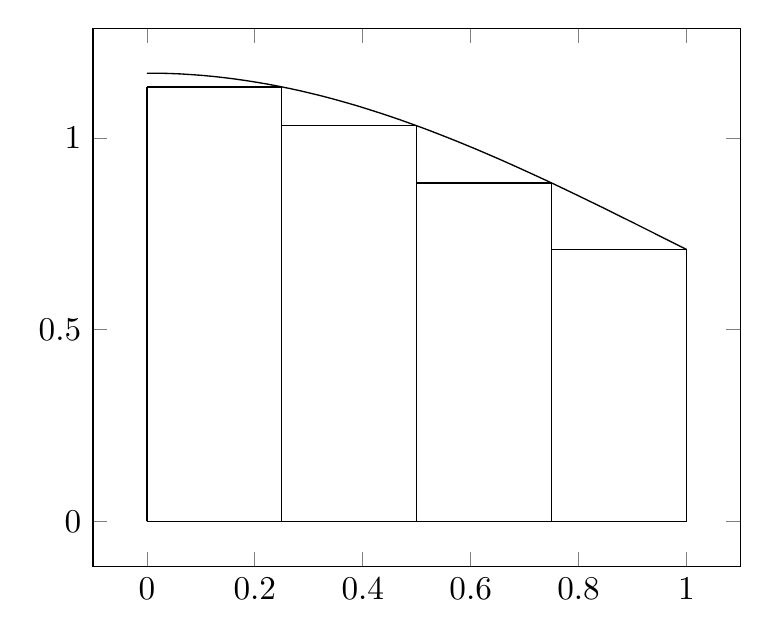
\begin{tikzpicture}[scale=1.2]
\begin{axis}
\addplot[draw=none] coordinates {(0,0)};
\addplot[domain=0:1,samples=50] {e^(-x^2/2)/0.855624};
\draw (axis cs: 0, 0) -- (axis cs: 1, 0);
\draw (axis cs: 0, 0) -- (axis cs: 0, 0.7088752307384394);
\draw (axis cs: 1, 0) -- (axis cs: 1, 0.7088752307384394);
\draw (axis cs: 0, 0) -- (axis cs: 0, 1.0314073738483691);
\draw (axis cs: 1/2, 0) -- (axis cs: 1/2, 1.0314073738483691);
\draw (axis cs: 1/2, 0) -- (axis cs: 1/2, 0.7088752311585824);
\draw (axis cs: 1, 0) -- (axis cs: 1, 0.7088752311585824);
\draw (axis cs: 0, 0) -- (axis cs: 0, 1.132779392052711);
\draw (axis cs: 1/4, 0) -- (axis cs: 1/4, 1.132779392052711);
\draw (axis cs: 0, 1.132779392052711) -- (axis cs: 1/4, 1.132779392052711);
\draw (axis cs: 1/4, 0) -- (axis cs: 1/4, 1.0314073740037737);
\draw (axis cs: 1/2, 0) -- (axis cs: 1/2, 1.0314073740037737);
\draw (axis cs: 1/4, 1.0314073740037737) -- (axis cs: 1/2, 1.0314073740037737);
\draw (axis cs: 1/2, 0) -- (axis cs: 1/2, 0.8822094784609293);
\draw (axis cs: 3/4, 0) -- (axis cs: 3/4, 0.8822094784609293);
\draw (axis cs: 1/2, 0.8822094784609293) -- (axis cs: 3/4, 0.8822094784609293);
\draw (axis cs: 3/4, 0) -- (axis cs: 3/4, 0.7088752308298532);
\draw (axis cs: 1, 0) -- (axis cs: 1, 0.7088752308298532);
\draw (axis cs: 3/4, 0.7088752308298532) -- (axis cs: 1, 0.7088752308298532);
\end{axis}
\end{tikzpicture}